%%%%%%%%%%%%%%%%%%%%%%%%%%%%%%%%%%%%%%%%%%%%%%%%%%%%%%%%%%%%%%%%%%%%%%%%%%%%
% AGUJournalTemplate.tex: this template file is for articles formatted with LaTeX
%
% This file includes commands and instructions
% given in the order necessary to produce a final output that will
% satisfy AGU requirements, including customized APA reference formatting.
%
% You may copy this file and give it your
% article name, and enter your text.
%
% guidelines and troubleshooting are here:

%% To submit your paper:
\documentclass[draft]{agujournal2019}
\usepackage{url} %this package should fix any errors with URLs in refs.
\usepackage{lineno}
\usepackage{placeins}
\usepackage{amsmath}
\usepackage{makecell}

\usepackage[inline]{trackchanges} %for better track changes. finalnew option will compile document with changes incorporated.
\usepackage{soul}
\linenumbers
%%%%%%%
% As of 2018 we recommend use of the TrackChanges package to mark revisions.
% The trackchanges package adds five new LaTeX commands:
%
%  \note[editor]{The note}
%  \annote[editor]{Text to annotate}{The note}
%  \add[editor]{Text to add}
%  \remove[editor]{Text to remove}
%  \change[editor]{Text to remove}{Text to add}
%
% complete documentation is here: http://trackchanges.sourceforge.net/
%%%%%%%

\draftfalse

\newcommand{\aref}[1]{\textbf{Reference #1}}
\newcommand{\TODO}[1]{\textbf{TODO: \color{red}#1}}
\newcommand{\ian}[1]{{\textbf{\color{blue}Ian says:} \color{blue} #1} }
\newcommand{\mauro}[1]{{\textbf{\color{green}Mauro says:} \color{green} #1} }
\newcommand{\alpine}{\textit{ALPINE}\,}
\newcommand{\icesheet}{\textit{ICESHEET}\,}
\newcommand{\m}{$\,\mathrm{m}$\,}
\newcommand{\cm}{$\,\mathrm{cm}$\,}
\newcommand{\mma}{$\,\mathrm{mm  \, a^{-1}}$\,}
\newcommand{\mmma}{$\,\mathrm{m^3\, a^{-1}}$\,}
\newcommand{\mmms}{$\,\mathrm{m^3\, s^{-1}}$\,}
\newcommand{\unit}[1]{$\mathrm{#1}$}

\journalname{Geophysical Research Letters}

\begin{document}

\title{Subglacial and subaerial fluvial sediment transport capacity respond differently to water discharge variations}

\authors{Ian Delaney\affil{1},  Andrew J. Tedstone\affil{2},   Mauro A. Werder\affil{3,4},  Daniel Farinotti\affil{3,4} }

\affiliation{1}{Institut des dynamiques de la surface terrestre (IDYST), Universit\'{e} de Lausanne, B\^{a}timent G\'{e}opolis, 1015 Lausanne, Switzerland}
\affiliation{2}{Department of Geosciences, University of Fribourg, Ch. du Musée 1700, Fribourg, Switzerland}
\affiliation{3}{Laboratory of Hydraulics, Hydrology and Glaciology (VAW), ETH-Z\"urich, H\"onggerbergring 26, 8093 89 Z\"urich, Switzerland}
\affiliation{4}{Swiss Federal Institute for Forest, Snow and Landscape Research (WSL) Z\"uricherstrasse 111, 8903 1011 Birmensdorf, Switzerland}

\correspondingauthor{Ian Delaney}{ianarburua.delaney@unil.ch}

change subglacial hydraulics to subglacial model outputs??

\begin{keypoints}
\item Short term water discharge variations in subglacial channels are mainly accommodated by water velocity, not channel size.
\item Greater variability in water velocity causes sediment transport capacity to vary more in subglacial channels than in subaerial channels.
\item Water discharge may represent processes including proglacial sediment mobilization and sediment access driving variations in sediment discharge, as opposed to subglacial sediment transport capacity in glacierized catchments. \mauro{I don't understand this sentence.}
\end{keypoints}

\begin{abstract}  Sediment transport capacity in subglacial and subaerial channels depends on  water velocity and channel width, which together control the total shear stress exerted on the channel bottom.
  In subaerial channels water discharge variations are accommodated largely by changes in flow depth and width.
  While in subglacial channels, water discharge changes primarily affect water velocity due to slow-evolving channel geometry.
  Parameterizations of these subglacial and subaerial hydraulics are applied to hydrographs from an Alpine glacier and the Greenland Ice Sheet revealing greater variability in the inferred sediment transport capacity in subglacial than in subaerial channels.
  Results show that high subglacial sediment transport rates can occur across a wide range of water discharges.
  Slowly evolving channel width accommodates some variability in subglacial channels. \mauro{not sure what that sentence should do}
  Despite differences in response to water discharge, sediment discharge measurements generally correlate better with subaerial hydraulic parameters.
  This implies that other factors like sediment access or proglacial processes might be at play that affect sediment transport capacity differently in subglacial and subaerial channels.
\end{abstract}

\section{Introduction}
\label{sect:intro}

Changes in glacier dynamics, geomorphology, and hydrology  have prompted numerous  recent studies of  sediment transport processes in cold regions \cite<e.g.>{zhang2022}.
Increases in sediment transport  have been observed in Greenland \cite{bendixen2017}, the European Alps \cite{costa2017}, the Himalayas \cite{li2021}, and the Andes \cite{vergara2022}.
In some regions, increased water discharge and glacier melt have been interpreted to yield greater sediment transport capacity \cite{bendixen2017,costa2017,li2021}.
Observed changes to sediment transport in glacierized catchments require examining the processes controlling sediment discharge in these catchments and its variations with water discharge  \cite<e.g.>{riihimaki2005,swift2005}.

Over long periods, processes such as glacier abrasion and quarrying sculpt landscapes and create sediment to be transported fluvially from under glaciers \cite<c.f.>{hallet1979,iverson2012,ugelvig2018}.
On shorter time periods, pressurized water transports sediment from underneath glaciers \cite{walder1994,creyts2013,beaud2018,delaney2019}, should enough sediment be present subglacially (i.e. in a transport-limited regime).

In a transport-limited regime, sediment discharge tracks sediment transport capacity, defined as the amount of sediment the water can carry.
Sediment transport capacity depends on the shear stress between water and the sediment it flows  over \cite{shields1936,meyer1948,engelund1967} along with the width of the channel bottom $w$ over which to mobilize sediment.
The shear stress $\tau$ responds to the velocity of water $v$ flowing through the channel so that
\begin{linenomath*}
  \begin{equation}
    \label{eq:tau}
    \tau_t \propto w\,v^2.
  \end{equation}
\end{linenomath*}
\mauro{I removed the width from here as I found it odd to introduce that here.}
%
Following mass conservation, the velocity of the water flowing through a  channel is
\begin{linenomath*}
  \begin{equation}
    \label{eq:v}
    v = \frac{Q}{S},
  \end{equation}
\end{linenomath*}
where $Q$ is water discharge,  and $S$ is the channel's wetted area. \mauro{I find it odd to have formulas in the Intro}

In subaerial channels, operating with open channel flow, the wetted area $S$ of the channel evolves with changing water discharge $Q$, by changing both the channel's width and the water depth \cite{leopold1953}.
The change in water depth results in a commensurate increase in water velocity.
%Thus,  fulfilling Equation~\ref {eq:v}, the higher discharge is accommodated by both an increase in wetted area and flow velocity. \mauro{not needed}
As a result, the shear stress $\tau$ increases according to Equation~\ref{eq:tau}.

The response of water velocity to changing water discharge in subglacial channels differs from subaerial ones.
The size of subglacial channels responds to the creep closure of the ice above and the opening of the channel by melting due to frictional heating of water flowing through the channel \cite{rothlisberger1972}.
As a result, the subglacial channel size only evolves relatively slowly over days to months, whereas water discharge can vary over hours \cite<e.g.>{iken1986,andrews2014,nanni2020}.
Therefore, on short time scales, subglacial water flow behaves more like pipe flow and changes in water discharge $Q$ are mainly accommodated with increased or decreased water velocity $v$ \cite{alley1997} because the size of the channel $S$ changes on a much longer timescale (Equation~\ref{eq:v} and Figure~\ref{fig:cartoon}).
%It follows that an increase in water discharge $Q$ will cause the shear stress across the channel $\tau_t$ to respond with water velocity $v$, as opposed to subaerial channels where channel width $w$ evolves as well.

  \begin{figure}[h]
  \centering
    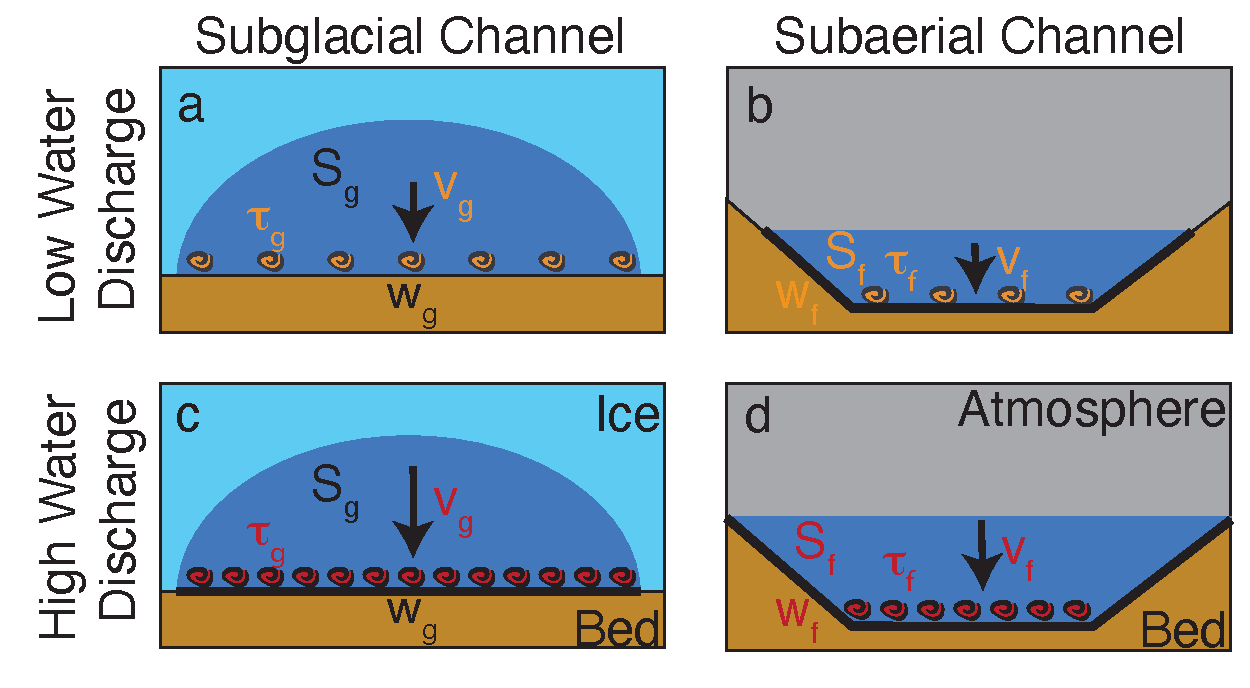
\includegraphics[width=0.8\linewidth]{Fig1.pdf}
    \caption{Sketch for the different responses that subglacial and subaerial channels to increased water discharge.
      Water velocity magnitudes in the subglacial, $v_g$, and subaerial, $v_f$, channels are shown by arrow length.
      $S_g$ and $S_f$ represent the wetted area in subglacial and subaerial channels, respectively.
      The subglacial channel widths $w_g$ remain unchanged, while the subaerial channel widths $w_f$ evolve. Shear stress $\tau$ is responsible for the mobilization of sediment.
      %Note that in the subaerial channel parameterization, channels have rectangular shapes with their width much larger than their depth (Section~\ref{sect:fluv}).
\mauro{Needs renaming $w_{cg/f}$ to $w_{g/f}$. Then, I find the downward arrow confusing.  Maybe just leave away? Also, I would write $\tau_f$ and $\tau_g$, it's ok to not have the width integrated tau here (and maybe we remove $\tau_{tf}$ from the paper anyway...}
    }
    \label{fig:cartoon}
  \end{figure}
% \ian{Come back to Daniel's comments}

Consequently, sediment mobilization in subaerial and subglacial channels responds differently to changing water discharge.
These differences are implicitly included in a wide range of available models that  quantify sediment transport in both subglacial and subaerial channels  \cite<e.g.>{walder1994,alley1997,tucker1997,creyts2013,delaney2019,hewitt2019,wickert2019}.
The divergent response of changing water discharge on sediment mobilization capacity may well impact sediment dynamics at glacier margins where flow transitions from pressurized to open channel flow \cite<e.g.>{perolo2018}.
Additionally, the variable response of sediment transport capacity to water discharge in the two systems may affect the interpretation of sediment transport records in glacial systems \cite<e.g.>{muller1968,richards2003,swift2005,ganti2016}.
Yet, little work has examined the differing relationship between variations in water discharge and sediment discharge in subglacial and subaerial channels \cite{alley1997}.
%Furthermore, thorough observations of water velocity and channel width in subglacial channels are limited and, to these authors' knowledge, not contrasted with subaerial conditions at the glacier margins. %\mauro{self-cite here?}

This manuscript evaluates the relationship between sediment transport capacity and water discharge in subglacial channels and compares it to subaerial ones.
Due to the absence of continuous measurements of subglacial and subaerial water velocity and channel morphology, numerical parameterizations of subglacial and subaerial hydraulics are utilized. \mauro{Aren't those things always parameterised, irrespective of whether there are measurements or not?}
Parameterizations are applied to hydrological records from an Alpine glacier in Switzerland (Fieschergletscher) and  a land-terminating glacier in Greenland (Leverett Glacier).
Our parameterizations' lumped nature isolates the disparity between water discharge and sediment transport capacity in subglacial systems, independent of the upstream drainage network and sediment access.
Outputs demonstrate differences in the relationships between  water discharge, channel geometry, and water velocity in the subglacial and subaerial channels.
Furthermore, outputs are compared to sediment discharge data from these two catchments.
The manuscript then uses the demonstrated differences between the two channel types to discuss the implications for interpreting the processes driving variability in records of sediment transport from glacierized catchments.
\mauro{As stated in the general comments.  I'd rather use ``model'' than ``parameterization'' as the latter is, for me, something which is used in a model and not a model itself.}

\section{Study sites and data}
\label{sect:ss_data}

Water and suspended sediment data are leveraged from Alpine and ice sheet settings.
The Alpine site (\alpine) is  Fieschergletscher in the Swiss Alps ($46^\circ\,29'\,07''$ N, $8^\circ\,08'\,3''$ E).
Water discharge and suspended sediment concentration were collected here at a $1$\unit{min} interval continuously over the period 2014--2021.
See \citeA{felix2022} and \citeA{felix2021} for more details.

The Leverett Glacier in Greenland (\icesheet) serves as the ice sheet setting.
Water discharge and suspended sediment concentration data were collected roughly $2$\unit{km} downstream from the terminus between June and August/September 2009 to 2012 ($67^\circ\,03'\,5''$ N, $50^\circ\,12'\,59''$ W).
Data is used from \citeA{tedstone2017} and \citeA{hawkings2014} at a $5$\,\unit{min} time interval from May 28, 2012 to August 8, 2012.
Two gaps (14.07.2012 to 15.07.2012 and 16.07.2012 to 17.07.2021) in suspended sediment data were interpolated using a linear spline.

\section{Methods}
\label{sect:meth}
The parameterizations below (Sections ~\ref{sect:sub_mode}~and~\ref{sect:fluv}) represent relationships amongst water discharge, water velocity, and channel geometry in both subaerial and subglacial channels (Table \ref{table:vpm}).
Both parameterizations calculate   water velocity, shear stress, and width-integrated shear stress, upon which sediment transport depends \cite<Figure \ref{fig:cartoon}; >{shields1936}.
The evaluation of these variables omits the selection of a sediment transport relationship and a grain-size parameter \cite<e.g.>{shields1936,meyer1948} needed to calculate sediment transport capacity from shear stress.


\subsection{Subglacial channel  parameterization}
\label{sect:sub_mode}

To evaluate the shear stress of water flowing across sediments underneath a glacier, the subglacial channel parameterization takes into account the channel geometry and the velocity of the flowing water.
To do this, a lumped hydraulics model \cite{clarke1996} modified from the one presented by \citeA{werder2010b} is used.

Here, it is assumed that the water is transported through a subglacial channel \cite<Figure~\ref{fig:cartoon}; >{rothlisberger1972}, and that the channel  size responds to melt due to frictional heating from water flow and to creep closure of the ice, using the Darcy-Weisbach formulation for water-flow through a pipe  \cite<e.g.>{rothlisberger1972,clarke2003}.
The formulation here does not consider the englacial storage of water.
Thus, it is assumed that the changing hydraulic head at the top of the glacier is negligible in the channel size evolution \mauro{I don't understand this sentence}.
The evolution of subglacial channel size $S_g$ is given as
\begin{linenomath*}
  \begin{equation}
    \label{eq:dS_dt}
    \frac{\partial S_g}{\partial t} = C_1 \frac{Q \Delta h}{l} - C_2 \left(h_{o}-\frac{\Delta h}{2}\right)^n\,S_g,
  \end{equation}
\end{linenomath*}
\noindent where $C_1= (1-\rho_wc_pc_t)\,\frac{\rho_wg}{\rho_iL}$ and $C_2=2A(\frac{\rho_wg}{n})^n$ are constants (Table \ref{table:vpm}), $l$ is the length of the subglacial channel, $Q$ is water discharge, $\Delta h$ is the hydraulic potential change from the glacier terminus to its top, $h_{o}= \frac{\rho_i}{\rho_w} h_{ice}$ is the ice overburden pressure expressed in meter water equivalent, and $n$ is Glen's n \cite{glen1955} (usually $n=3$).
The first term on the right side of the equation represents the opening of the channel through frictional heating, while the following term represents the creep closure of the channel from ice deformation.


Following the Darcy-Weisbach equation, the head drop $\Delta h$ is
\begin{linenomath*}
  \begin{equation}
    \label{eq:dh}
    \Delta h \,  = l \,\frac{1}{2g} \,f_r\,\frac{v_g^2}{D_h},
  \end{equation}
\end{linenomath*}
\noindent where $f_r$ is a friction factor, $D_h$ is the hydraulic diameter, $l$ is the length over which head change occurs, and $v_g=Q/S_g$ is the water flow speed.
%
The hydraulic diameter $D_h$ is converted to wetted area $S_g$ with
\begin{equation}
  \label{eq:Dh2S}
  S_g= \frac{D_h^2}{2}\,\frac{(\frac{\beta}{2}+\sin \frac{\beta}{2})^2}{\beta - \sin \beta},
\end{equation}
where $\beta$ is the central angle of the circular segment that comprises the channel (the so-called Hooke angle, \citeA{hooke1990}). Note that $\beta =\pi$ corresponds to a semi-circular channel and smaller values of $\beta$ result in shallow, wide channels.
%
The shear stress, $\tau_g$, between the water and the channel bed is determined through the Darcy-Weisbach formulation
\begin{equation}
  \label{eq:tau}
  \tau_g=\frac{1}{8}\,f_r\,\rho_w\,v_g^2,
\end{equation}
%
where $v_g = \frac{Q}{S_g}$ is the water velocity.
%
The width-integrated shear stress is represented as
\begin{equation}
  \label{eq:tautg}
  \tau_{tg}=w_g\,\tau_g,
\end{equation}
where  channel floor width $w_g$ is
\begin{equation}
  \label{eq:dh2wc}
  w_g = 2  \sin \frac{\beta}{2} \sqrt{\frac{2\, S_g}{\beta -\sin \beta}}.
\end{equation}
\mauro{If we get rid of $\tau_{tf}$, above needs a bit of massaging.  I'd then move the $w_g$ eq to just after the $S_g$ eq.}

\subsection{Subaerial channel  parameterization}
\label{sect:fluv}

% To parameterize the shear stress of water flowing across sediments in the subaerial channel, the hydraulics parameterization presented in \citeA{tucker1997} is implemented.
Using mass conservation and the Darcy-Weisbach relationship as well as assuming that the channel is wide so that the hydraulic radius is well approximated by the flow depth, then
the shear stress $\tau_f$ at the river bed is
\begin{linenomath*}
  \begin{equation}
    \label{eq:DW_tau}
    \tau_f=\frac{\rho_w\,g^{\frac{2}{3}}\,f_p^{\frac{1}{3}}}{2}\, \Big(\frac{Q}{w_f} \Big)^{\frac{2}{3}} \,\nabla z_c^{\frac{2}{3}},
  \end{equation}
\end{linenomath*}
where $\nabla z_c$ is the channel slope, and $f_p$ is the friction factor for subaerial channels \cite{tucker1997}.
Channel width $w_f$ is
\begin{equation}
  \label{eq:wcf}
  w_f = k \, Q^{\alpha},
\end{equation}
%
where $k$ is a constant and $\alpha=\frac{1}{2}$ is a commonly chosen exponent \cite{leopold1953}.
Water velocity, $v_f$, is given by rearranging Equation \ref{eq:tau} as
\begin{equation}
  \label{eq:vf}
  v_f = \sqrt{\frac{8\,\tau_f}{f_p\,\rho_w}}.
\end{equation}
%
As above, the width-integrated shear stress is
\begin{equation}
    \label{eq:tautf}
    \tau_{tf}=w_f\,\tau_f.
  \end{equation}

  Note that the subaerial channel model \mauro{or ``parameterization''} is a purely algebraic model, whereas the subglacial model comprises a differential equation for the evolution of $S_g$ and thus will have a history dependence on the discharge.

\subsection{Implementation}
\label{sect:imp}

\mauro{I would call the ``cases'' ``scenarios'' instead.  The word ``scenario'' does not appear in the manuscript so far, so it would be unambiguous.  Also, ``cases'' has the disadvantage that ``In both cases,'' is a saying, and thus it is confusing.  I implemented this change.}

The parameterizations above are applied to hydrological records from the Fieschergletscher (scenario \alpine) and the Leverett Glacier (scenario \icesheet).
The subglacial and subaerial parameterizations represent the subglacial flow of water exiting a glacier and transitioning to subaerial flow.
Outputs of the parameterizations represent generalizable sediment transport characteristics from these hydrographs, rather than actual hydraulic conditions.
To generalize these scenarios, \alpine{}  is exemplified by relatively thin ice thickness ($h_{ice}$: $225$\,\unit{m}), low water discharge ($\sim\,10$\,\unit{m}$^3$\,\unit{s}$^{-1}$) and high diurnal variability in water discharge (Figure~\ref{fig:model_outs}, a).
\icesheet{}  is exemplified by thick ice  ($h_{ice}$: $700$\,\unit{m}), high water discharge ($\sim\,300$\,\unit{m}$^3$\,\unit{s}$^{-1}$)  and low diurnal variability in water discharge (Figure~\ref{fig:model_outs}, e).
%
However, both scenarios share a discharge with a similar, relative seasonal amplitude.

For each glacier, the parameterizations are first applied to a reference test case for each glacier that assumes  a subglacial channel with $\beta=\frac{\pi}{2}$, i.e. a segment of a quarter-circle.
Friction factors $f_r$ and $f_p$ are tuned so that the parameterizations reproduce reasonable water velocities for both \alpine and \icesheet{}\cite<$\sim\,1.6\,$\unit{m}$^3$\,\unit{s}$^{-1}$>{werder2010b,chandler2013}.
\mauro{Those $f$ reported in the table are super large!  Maybe an issue down the line...}
The subaerial channels of both scenarios have a bed slope of $\nabla z_c = 0.05$ \mauro{Why do you report a value here but most are hidden in the table?  Maybe just ref the table?}.
% Water velocity, shear stress, and width-integrated shear stress in the subglacial and subaerial channels from this formulation are presented below.

Second, to further characterize the variability in sediment discharge capacity in subglacial compared to subaerial channels, $100$  parameter combinations are applied to a range of different channel geometry factors ($\beta$ and $k$) and friction factors ($f_r$ and $f_p$). \mauro{So how many runs are actually run?  Not clear.}
Runs with parameter combinations are culled if their mean subglacial water velocity over the season lies outwith $0.75$\,\unit{m}$^3$\,\unit{s}$^{-1}$ and $2$\,\unit{m}$^3$\,\unit{s}$^{-1}$ or if subaerial water velocity lies outwith $0.3$\,\unit{m}$^3$\,\unit{s}$^{-1}$ and $1.2$\,\unit{m}$^3$\,\unit{s}$^{-1}$, in accordance with measurements \cite<e.g.>{werder2010b,magnusson2012,chandler2013} \mauro{Awkward sentence.  (also note that ``cull'' means to remove, thus I changed ``between'' to ``outwith''.}.
The variability of output is represented by the  standard deviation of that output over the course of the season \mauro{This sentence needs context.  What is variability used for?}.

Lastly, outputs of $w\tau$ are compared with the sediment discharge records of the glaciers using Spearman rank correlation, dependent on the ordering of values.
Rank correlation reduces the impact of the non-linear response of sediment transport capacity to the hydrological forcing, thus making our interpretation independent of the exact details of the sediment transport formula.
Outputs and observations, which have a $15$\,\unit{min} resolution, are aggregated across time intervals of up to $15$\,\unit{days} by averaging values over a symmetric window of corresponding size.

\section{Results}

\subsection{Role of water discharge in sediment transport capacity}
\begin{figure}[h]
  \centering
  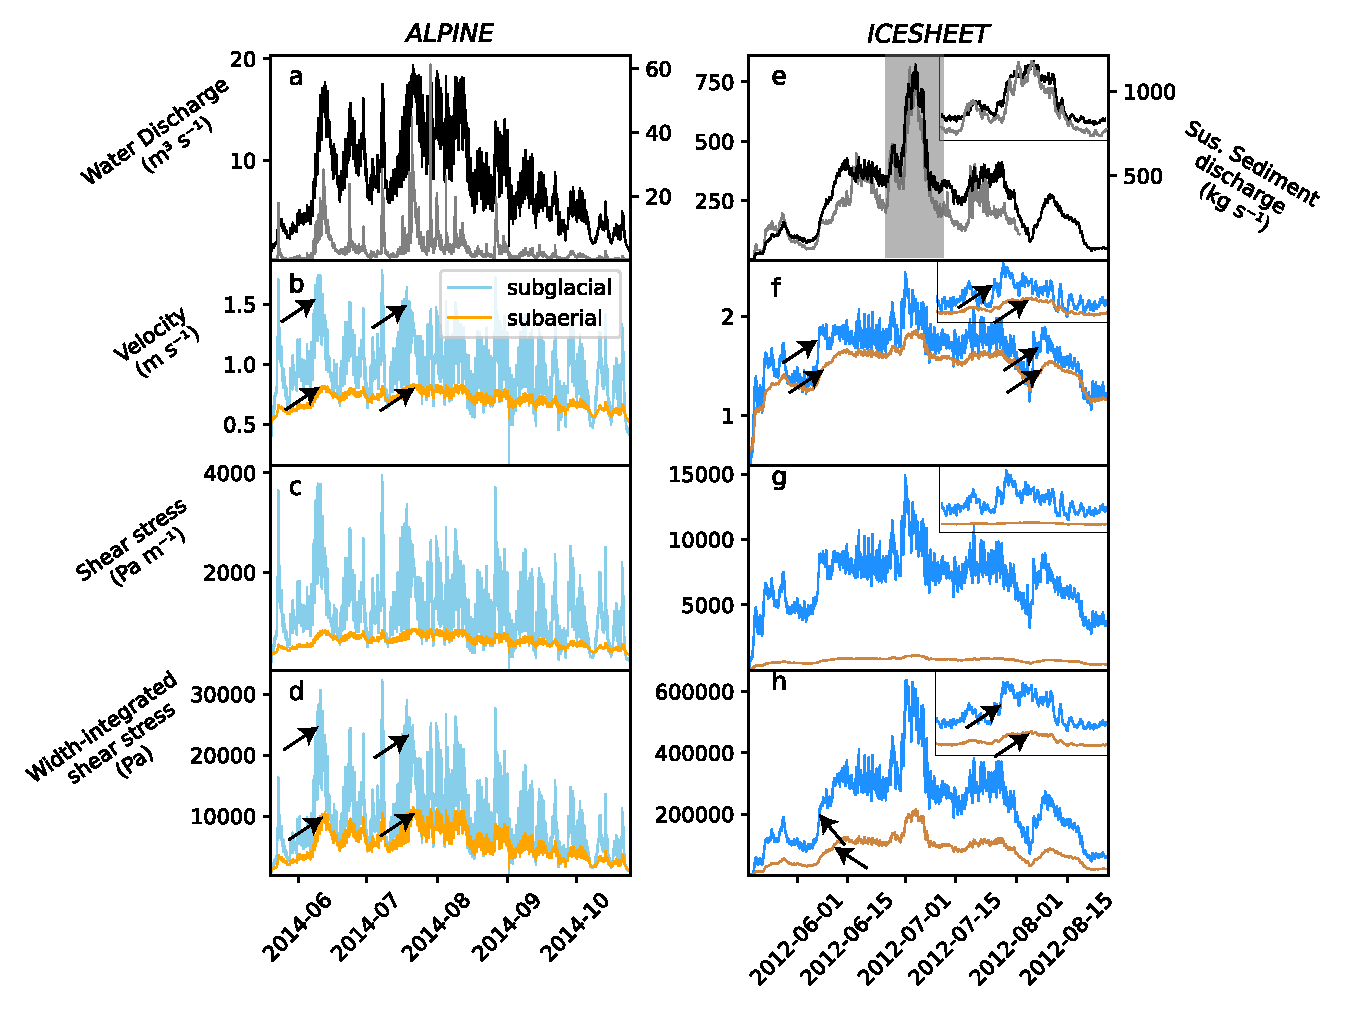
\includegraphics[width=0.9\linewidth]{Fig2.pdf}
  \caption{Parameterization outputs from the hydrographs n panels a and e for \alpine scenarios (a-d) and \icesheet{} (e-h).
    Gray (black) lines in a and e represent the subglacial channel size (water discharge).
    Blue lines represent outputs from the subglacial channel, while orange lines represent the subaerial channel.
    Data are shown at $15$\unit{min} intervals, i.e. not aggregated.
    Arrows denote where variables peaking in the subglacial channel prior to the subaerial one \mauro{wouldn't this need more zoomed-in plots?}.
    Insets in e-h show the  peak melt event \icesheet{} denoted by the shaded area in panel e.
    % Note that the x and y axes are different for \alpine{} and \icesheet{}.
        \mauro{Wrong units! Shear stress is Pa\,m$^{-2}$ and width integrated Pa\,m$^{-1}$}
  }
  \label{fig:model_outs}
\end{figure}

\mauro{Good para}
Following the parameterizations defined in Sections~\ref{sect:sub_mode}~and~\ref{sect:fluv}, the water velocity, shear stress, and width-integrated shear stress exhibit different seasonal evolutions and peaks.
Water velocity and shear stress represent the potential for sediment mobilization, and width-integrated shear stress represents a proxy for the total sediment transport capacity across the channel bed (Figure~\ref{fig:model_outs}).

\mauro{In principle good paragraph, the meat.  But suffers from sloppy writing.}
In the subglacial channel, peaks in $w_g\tau_g$ generally occur when water discharge increases at the fastest rate (Figure~\ref{fig:model_outs}d,h).
In contrast, in the subaerial channel,   $w_g\tau_g$  peaks when water discharge is highest.
The timing of the greatest rate of change in water discharge occurs before the peaks in water discharge \mauro{what?}.
Furthermore, the subglacial outputs \mauro{What are ``outputs''?}  are generally larger than the subaerial values, thus more efficient at transporting sediment.
Here, sediment could be deposited in the proglacial area as the water depressurizes, then remobilized when sediment transport capacity peaks in the subaerial system \mauro{not sure this tangent is worth taking in this paragraph}.

\begin{figure}[h]
  \centering
  \includegraphics[width=0.9\linewidth]{Fig3.png}
  \caption{
    Relationship between water discharge and velocity, shear stress, and width-integrated shear stress for \alpine{} (a-c) and \icesheet (d-f).
    These outputs' relationship with measured sediment discharge is given for \alpine in (g-i) and \icesheet (j-l).
    Variables on the x-axis have been normalized to mean values.
    $R_g$ and $R_f$ show the Spearman rank correlations for the subglacial and the subaerial outputs, respectively.
    Plots are shown with data and outputs at $15$\unit{min} intervals.
    \mauro{Pixely, needs more resolution, at least 2x. The two dots in the legend are not visible.  I would add ``Measured'' to the two y-labels.}
  }
  \label{fig:Qw_vari}
\end{figure}

In the subaerial system there is no history dependence and thus each water discharge value in the subaerial channel results in a unique water velocity, shear stress, and width-integrated shear stress, creating a perfect rank correlation between the variables (Figure~\ref{fig:Qw_vari} a--f).

\mauro{it feels this sentence should be in the same para as the previous one.  But not sure what it tries to say.}
In the subglacial channel, however, the persistence of high water velocity, shear stress, and width-integrated shear stress across a range of discharges suggests that substantial sediment transport may occur across \mauro{across what?} (Figure~\ref{fig:Qw_vari} a--f).



For instance, very high  water velocity values and shear stresses can occur across minimal water discharge at $2.5$\,\unit{m}$^3$\,\unit{s}$^{-1}$ to the maximum water discharge at over $17$ \,\unit{m}$^3$\,\unit{s}$^{-1}$.
In \icesheet, mean values \mauro{what ``mean''?} of water velocity can occur at water discharges between roughly $150$ \,\unit{m}$^3$\,\unit{s}$^{-1}$ and $310$ \,\unit{m}$^3$\,\unit{s}$^{-1}$.
When considering the subglacial channel's evolving width, width-integrated shear stress  across the channel generally increases with water discharge, with improved rank correlation compared to water velocity or shear stress (\alpine, Figure~\ref{fig:Qw_vari} a--f).
Yet even the width-integrated shear stress  can vary substantially, with the highest values occurring at water discharge values ranging from roughly $11$ \,\unit{m}$^3$\,\unit{s}$^{-1}$ to over $17$ \,\unit{m}$^3$\,\unit{s}$^{-1}$.
The variability in width-integrated shear stress is less pronounced in the \icesheet scenario, with reduced variability in water discharge (Figure~\ref{fig:Qw_vari} c, f).

\begin{figure}[h]
  \centering
    \includegraphics[width=0.9\linewidth]{Fig4.png}
    \caption{Variability (standard deviation) of output variables for different time aggregations across the range of subglacial and subaerial channel shapes and friction factors.
      Shaded areas denote the range of the $100$ parameter combinations tested (Section~\ref{sect:imp}).
      Solid lines denote  mean values.
      %Top row shows results from the \alpine{} scenario, while bottom row show outputs from the \icesheet{} scenario
      Time intervals shown with markers denote $15$\,\unit{min}, $1$\,\unit{hr}, $12$\,\unit{hr}, $1$\,\unit{d}, $5$\,\unit{d}, $10$\,\unit{d}, and $15$\,\unit{d} aggregation periods.
      Text in columns shows rank correlation between the variable and sediment discharge for the corresponding time period for the subglacial (left column) and subaerial (right column) channels.
      \mauro{Again units are wrong as in Fig 2.
        I would add \alpine and \icesheet labels to the plots; and for sure that needs to be stated in the caption.
        It's a bit confusing to have the rank-correlations here as well as they are not on the variability but just on the variable themselves... not sure what to do though. } }
    \label{fig:multi_run}
  \end{figure}

Across the range of channel shape parameters and friction factors  examined, variability in water velocity and shear stress remains higher in the subglacial system compared to the subaerial one.
In \alpine{}, the variability in width-integrated shear stress is comparable between the two systems, due to the variable water discharge (Figure~\ref{fig:multi_run}).

However, in \icesheet{}, with lower water discharge fluctuations, the variability in width-integrated shear stress remains higher in the subglacial system across the time aggregation periods.

\mauro{this paragraph needs more motivation: why are we looking at this?}
It is prescient \mauro{I don't think that works ``to have foresight''} to evaluate the time scales over which the subglacial channels may respond to changing water discharge to understand the influence of variability in sediment transport capacity.
In both scenarios, the variability in velocity, shear stress, and width-integrated shear stress decreases with aggregations longer than approximately 1--5 days (Figure~\ref{fig:multi_run}).
Yet, substantial differences in variability persist in periods of up to $15$ days.
Aggregations periods longer than this might be conflated with seasonal variations in water discharge and are thus omitted.
Note that lags and time of peak sediment transport conditions still occur over these periods (Figure~\ref{fig:model_outs}), while the variability in sediment transport parameters decreases with larger time aggregation (Figure~\ref{fig:multi_run}) \mauro{not clear sentence}.


\subsection{Relationship between parameterization  outputs and observed sediment discharge}
\mauro{Not sure a separate section is needed for this one paragraph.}

When comparing the outputs with suspended sediment discharge measurements, the subaerial parameterizations generally correlate better with sediment discharge compared to subglacial outputs across the tested parameters (Figures~\ref{fig:Qw_vari} g--l and \ref{fig:multi_run}).
The rank correlation amongst the subaerial parameterization's outputs remains fairly constant despite the variable impact of channel shape and consistent scaling with water discharge (Figure \ref{fig:Qw_vari} and Section~\ref{sect:fluv}).
In subglacial channels, velocity and shear stress perform substantially worse in terms of rank correlation with sediment discharge compared to width-integrated shear stress (Figures~ \ref{fig:multi_run}).
In both \alpine{} and \icesheet{}, the subglacial rank correlation approaches that of subaerial channels over longer time aggregation periods (Figures~ \ref{fig:multi_run} and \ref{fig:model_outs_1hr} to \ref{fig:model_outs_15day}).


\section{Discussion}
\subsection{Sediment capacity differences between the channel types}
\label{sect:dis_qsc}

Quantities that relate to sediment transport capacity (water velocity, shear stress, and width-integrated shear stress) vary differently in response to water discharge in subglacial channels compared to subaerial ones (Figure~\ref{fig:Qw_vari}).
In sediment transport relationships that evaluate sediment discharge capacity, such as in \citeA{meyer1948} or \citeA{engelund1967}, shear stress is scaled to the power of $\frac{3}{2}$ or $\frac{5}{2}$, respectively.
The exponent greater than $1$ magnifies sediment discharge variability beyond the variable sediment transport parameters described above (Figure~\ref{fig:multi_run}; Table~\ref{tab:Qs}).
Note that sediment transport relationships describe sediment flux per unit width, so that the integrated capacity across channel occurs after application of the exponent, unlike the width-integrated shear stress evaluation here \cite<Equations\,\ref{eq:tautg} and \ref{eq:tautf}; c.f.>{tucker1997} \mauro{sentence does not parse; I think you should state limitations of width integrated shear stress and then be done with it.}.
%Note also that both subglacial and subaerial parameterizations here assume that the distribution of velocity and shear stress is homogeneous across the channel bed, despite the limitations of this assumption \cite<e.g.>{yager2018}.

\mauro{This paragraph needs rewriting.  I guess I should do that.}
The rapid increases and decreases in subglacial sediment transport capacity compounds the variability in sediment transport already present in subaerial systems \cite<Figure~\ref{fig:Qw_vari}; >{williams1989,jerolmack2010}.
Sediment transport capacity in subglacial channels responds more rapidly to changes in water discharge compared to their subaerial counter parts \cite{alley1997}.
In subglacial R\"othlisberger channels in steady state with respect to water discharge the width-integrated shear stress response to water discharge is $ \tau_{tg}\, \propto\,  Q^{\sim\frac{4}{5}}$ (Table\,\ref{tab:eqs1}).
However, subglacial channels rarely operate in a steady state \cite<e.g.>{gimbert2016}.
For sufficiently short time periods, channel width and wetted area are fixed in the subglacial system (akin to pipe flow) so that the response of width-integrated shear stress is $ \tau_{tg}\, \propto\,  Q^{2}$ (Table\,\ref{tab:eqs1}).
\ref{sect:scaling} provides a complete description of sediment transport capacity in different drainage conditions.

\mauro{You often use ``subglacial hydraulics''.  I'm not sure what that means. For instance in the next sentence.  Isn't discharge part of hydraulics too?  Maybe you could define a bunch of equations as the subglacial hydraulic model and subaerial hydraulic model and then talk of that?}
%
The stronger correlation between subglacial hydraulics and water discharge in \icesheet{} (Figure~\ref{fig:Qw_vari}\,a-f) could result from the channel being closer to equilibrium between variations in the channels' wetter area and water discharge with smaller diurnal variations in amplitude (Figures~\ref{fig:model_outs} and ~\ref{fig:Qw_vari}) \mauro{needs rewriting}.
Conversely, the correlation between hydraulics and water discharge in \alpine is smaller due to the relatively larger discharge variations on short time scales.
In both scenarios, the variability in subglacial channels approaches that of subaerial ones  over $1-5$ days (Figure~\ref{fig:multi_run}), suggesting a parity between the two channel types might be approached over this period.

In subglacial channels, peaks in water velocity, shear stress and width-integrated shear stress occur with  fast rates of water discharge increase relative to the channel's growth rate (Figure~\ref{fig:model_outs}).
In turn, subglacial channels grow with increasing water discharge, effectively reducing sediment transport capacity with the stabilization of water discharge at its peak.
Similar feedback occurs in subaerial systems \cite{phillips2016}, albeit at timescales longer than days in the subglacial system.  

\subsection{Effect of variable sediment transport capacity on sediment discharge  from glaciers}
\mauro{This section header sounds like this will be about measurements only.}

\mauro{I find this confusing.  The measurements are sediment discharge, so how can they be represent by hydraulic outputs?  Maybe talk of sediment discharge proxy ($w\tau$) or some such?  Or use something establishing a less direct link than ``representing''.}
The increased performance of subaerial hydraulics outputs, compared to subglacial ones, in representing observations occurs despite the proximity of measurement locations to these glaciers (Figure~\ref{fig:Qw_vari}).
This could occur for two reasons.

First, these measurement stations lie $0.5$ to $2$\,\unit{km} downstream of the glacier terminus \cite{cowton2012,felix2022}, a long enough distance for the pressurized subglacial regime to transition to the open channel subaerial one.
The transition of subglacial to subaerial conditions typically occur still underneath glacier but close to the terminus \cite{perolo2018}, where closure rates of the subglacial channels are slow and open channel flow condition prevail \cite{rothlisberger1972}.
Furthermore, if abundant sediment persists in the proglacial area, then it can be easily mobilized, and subaerial processes could be represented just a short distance downstream \mauro{Not sure what that sentence means}.

\mauro{I perceived this paragraph pretty out of the blue.}
The consistent relationship between sediment discharge capacity in  open channel flow conditions could be pronounced $\sim20$\,\unit{km} downstream of the Leverett site, where a strong correlation persists between sediment plume size and the river's water discharge into the Kangerlussuaq fjord \cite{mcgrath2010}.
In contrast, in marine-terminating glacier catchments a less consistent relationship may occur between water discharge or melt extent and sediment plume size \cite{tedstone2012}.
Here, ocean water pressurizes subglacial channels at the ice front \cite<e.g.>{how2017}, so the minimal correlation could result from the inconsistent relationship between subglacial sediment transport capacity and water discharge (Figure~\ref{fig:Qw_vari}).

Second, the sediment discharge records could represent processes such as increased sediment accessibility when melt extends up the glacier, thereby increasing sediment and water discharge \cite<e.g.>{vergara2022}.
A supply-limited regime could well persist at many glaciers, because the sediment's threshold of motion can be reached more frequently and across a range of water discharges, compared to subaerial systems (Figure~\ref{fig:Qw_vari}).
Sediment exhaustion occurring through increased variability may also explain the stronger dependence of sediment discharge from the Greenland Ice Sheet on basal shear stress, a proxy for bedrock erosion, rather than glacier melt \cite{overeem2017}.
Note, however, the absence of lags between the observed sediment and water discharge (Figure~\ref{fig:model_outs}\, a and e) may suggest that sediment is mobilized close to the measurement stations, as opposed to distal areas of the glacier bed as would be expected in a supply-limited regime \cite{williams1989}.

Regardless of the increased performance of water discharge compared to subglacial sediment transport capacity in representing the observations,  suggest that additional processes and erosional hiatuses may further complicate signals of sediment discharge from glaciers in response to climate \cite{jansson2005,ganti2016}.
Sediment discharge records have been used to establish the relationship, or lack thereof, between climate forcing and glacial erosion \cite<e.g.>{koppes2009a,ganti2016,willenbring2016,mariotti2021}.
The variable relationship between water discharge and subglacial sediment transport capacity presented here mostly applies to the daily- to weekly-time scales controlling the size of subglacial channels (Figure~\ref{fig:multi_run}).
Yet, identifying climatic effects in sediment transport from the transport-limited component of glacier-sedimentary systems may require higher thresholds of water discharge compared to subaerial systems when water discharge varies substantially over short timescales \cite<Figure~\ref{fig:Qw_vari}; >{tofelde2021}. \mauro{I don't understand the last two sentences.}

Over time scales of weeks or longer, the glacier's sediment transport capacity is impacted by the ice thickness, controlling the channel closure rate, and the glacier's surface slope, in addition to water discharge \cite<Figure~\ref{fig:multi_run}, Section~\ref{sect:sub_mode}; >{rothlisberger1972,shreve1972,gimbert2016,stevens2022}.
In a supply-limited state, often assumed in landscape evolution models, then glaciers' sediment discharge record are also impacted by the additional processes of sediment availability and bedrock erosion from  water pressure variations and sliding  \cite<e.g.>{iverson2012,herman2015,delaney2023}.
This multitude of processes lies in contrast to processes occurring in most subaerial systems, where transport capacity typically responds to sediment size, water discharge, and hydraulic gradient, and the hydraulic gradient generally remains stable over time scales ranging from years to millennia \cite<Section~\ref{sect:fluv}; e.g.>{muller1968,tucker1997,wickert2019}.
The stronger link between sediment transport capacity and hydrological forcing in subaerial channels may mean that variations in sediment transport records can be more easily attributed to climatic conditions than in subglacial systems.


\ian{move this shit up or delete}
\subsection{Comparison of Alpine and Arctic hydrological forcing}

\section{Conclusions}

The sediment transport capacity of a channel is driven by its width and the shear stress exerted by the flowing water, which, in turn, is proportional to the square of the flow velocity.
Subaerial channels alter both their channel width and water velocity immediately in response to changing water discharge.
In contrast, pressurized subglacial channels largely accommodate rapidly changing water discharge by altering water velocity.
Their size, in contrast, responds over the course of several days to changes in discharge.
Thus the response of sediment transport capacity is much more sensitive to changes in water discharge in subglacial channels compared to subaerial ones.
%Despite these differences, parameterizations of subaerial hydraulics in two glacierized catchments generally represent observed sediment discharge variations better than subglacial hydraulics \mauro{This sentence does not quite parse.  Why ``despite''?  Also state that we found this.}

Implications of the presented findings include:
\begin{enumerate}
\item the changing relationship between water discharge and sediment transport capacity underneath glaciers creates larger variability in sediment transport capacity compared to river systems;
\item the timing of peak sediment transport capacity below glaciers generally coincides with large rates of increase in water discharge, as opposed to the maximum water discharge, as would occur in pipe flow of a fixed size;
\item the timing of peak sediment transport capacity in subaerial channels coincides with the maximum water discharge;
\item a steady relationship between water and sediment discharge may represent subglacial sediment access or open channel hydraulics near the glacier margin, instead of subglacial sediment transport capacity.
\end{enumerate}

\section*{Author Contributions}

I.D. designed the study, developed, and implemented the model and experiments, and wrote the manuscript.
A.J.T. helped interpret data from Leverett Glacier and provided guidance on experiment design.
M.A.W. provided data from Fieschergletscher and added the relationship between shear stress and water discharge (see Sections~\ref{sect:dis_qsc} and \ref{sect:scaling}).
D.F. provided data from Fieschergletscher.
All authors provided  key inputs in writing and editing the manuscript.


\section*{Open Research Section}

Code to make the figures, with links to the data, can be found at \url{https://bitbucket.org/IanDelaney/xsection/src/master/}.
Code and data will be uploaded to a permanent repository, with FAIR principles, pending acceptance of the paper.

\acknowledgments

SNSF Project No. PZ00P2\_202024 provided  funding for I. Delaney.
A. Tedstone acknowledges funding from the European Research Council, award 818994 -- CASSANDRA.
G. King provided useful comments on a previous version of this manuscript.


\bibliography{PaperLib}

\newpage

\appendix
\section{Table of variables, parameters and constants}
\begin{table}[h]
  \centering
  \caption{Variables, parameters, and constants used in this work.
    Where two values are given, the first refers to  \alpine{}, a scenario from Fieschergletscher, and the second to a glacier marginal to the \icesheet{} a scenario from Leverett Glacier}
  \tiny % TODO remove again
  \begin{tabular}{ l  c  c c }
    Name &Symbol&  Value&Units \\
    && (\alpine or \icesheet)\\
    \hline
    \textbf{Variables}  & & & \\
    Water discharge  & $Q$& & $\mathrm{m^{3}\,s^{-1}}$ \\
    Water velocity (subglacial, subaerial)  & $v$, ($v_g,\,v_{f}$)& & $\mathrm{m\,s^{-1}}$ \\
    Channel wetted area (subglacial, subaerial) &  $S_g, S_f$& & $\mathrm{m^2}$     \\
    Channel depth (subaerial) & $H$&& $\mathrm{m}$\\
    Hydraulic diameter &$D_h$&&$\mathrm{m}$\\
    Width of channel floor (subglacial, subaerial) & $w$, ($w_g,w_f$)&  & $\mathrm{m}$     \\
    Hydraulic head &$\Delta h$&& $\mathrm{m}$\\
    Hydraulic gradient &$\Psi=\frac{\Delta h}{l}$&& $\mathrm{m\, m^{-1}}$\\

    Shear stress (subglacial, subaerial) & $\tau$, ($\tau_g,\,\tau_f$) && $\mathrm{Pa \, m^{-2}}$ \\
    Width-integrated shear stress (subglacial, subaerial) \mauro{get rid of this} & $\tau_{tg},\, \tau_{tf}$&& $\mathrm{Pa \, m^{-1}}$\\
    Stream power & $\Omega$ && $\mathrm{ kg \, m\, s^{-3}}$ \\

         &&&\\

    \textbf{Parameters and Constants}  & & &\\
    Gravitational constant&$g$& $9.81$&$\mathrm{m\,s^{-2}}$\\
    Density of water & $\rho_w$& $1000$ & $\mathrm{kg\,m^{-3}}$ \\
    Density of ice & $\rho_i$& $900$ & $\mathrm{kg\,m^{-3}}$ \\
    Hooke angle of channel & $\beta$ & $\frac{\pi}{2}$ & \unit{rad}\\
    Glacier thickness &$h_{ice}$& $225$ or $700$  &\unit{m}\\
    Effective glacier thickness &$h_o$&$\frac{\rho_i}{\rho_w} h_{ice}$  &\unit{m}\\
    Effective glacier length &$l$& 7,000 or 26,000&\unit{m}\\
    Constant $1$ in Equation~\ref{eq:dS_dt} &$C_1$&$2.2\times10^{-5}$&\unit{m}$^{-1}$\\
    Constant $2$ in Equation~\ref{eq:dS_dt} &$C_2$&$3.7\times10^{-13}$&\unit{m}$^{-n}\,s^{-1}$\\
    Latent heat of fusion &$L$&$333.5 $&\unit{kJ\,kg}$^{-1}$\\
    Pressure melting coefficient &$c_t$&$7.5\times 10^{-8}$&\unit{K\,Pa}$^{-1}$\\
    Specific heat capacity of water &$c_p$&$4180$&\unit{J\,kg}$^{-1}$\unit{K}$^{-1}$\\
    Ice flow constant &$A$& $5.3\times10^{-24}$ &\unit{Pa}$^{-n}$\,$s^{-1}$\\
    Ice flow exponent &$n$& $3$ &$\mathrm{(-)}$\\
    Friction factor (subglacial, subaerial)  \mauro{why not $f_g$ and $f_f$?} & $f_r$ &$10$ or $20$ & $\mathrm{(-)}$ \\
    Friction factor (subaerial) & $f_p$ & $3$ & $\mathrm{(-)}$\\
    Gradient of channel bed (subaerial) &$\nabla z_c$ &$0.05$& $\mathrm{(-)}$\\
    Subaerial channel factor & $k$ &$3$ or $6.5$ & $\mathrm{s\,m^{-2}}$\\
    Channel geometry exponent &$\alpha$& $\frac{1}{2}$&$\mathrm{(-)}$ \\
    \hline
  \end{tabular}
  \label{table:vpm}
\end{table}
\FloatBarrier

\section{Figure 3 over various time aggregations}

\begin{center}
  \begin{figure}[!h]
    \includegraphics[width=0.7\linewidth]{Fig3_hr.png}
    \caption{As Figure \ref{fig:model_outs}, with $1$ \,\unit{hr} aggregation.}
    \label{fig:model_outs_1hr}
  \end{figure}
\end{center}

\begin{center}
  \begin{figure}[!h]
    \includegraphics[width=0.7\linewidth]{Fig3_12hr.png}
    \caption{As Figure \ref{fig:model_outs}, with $12$ \,\unit{hr} aggregation.}
    \label{fig:model_outs_12hr}
  \end{figure}
\end{center}


\begin{center}
  \begin{figure}[!h]
    \includegraphics[width=0.7\linewidth]{Fig3_1day.png}
    \caption{As Figure \ref{fig:model_outs}, with $1$ \,\unit{day} aggregation.}
    \label{fig:model_outs_1day}
  \end{figure}
\end{center}


\begin{center}
  \begin{figure}[!h]
    \includegraphics[width=0.7\linewidth]{Fig3_5day.png}
    \caption{As Figure \ref{fig:model_outs}, with $5$ \,\unit{day} aggregation.}
    \label{fig:model_outs_5day}
  \end{figure}
\end{center}

\begin{center}
  \begin{figure}[!h]
    \includegraphics[width=0.7\linewidth]{Fig3_10day.png}
    \caption{As Figure \ref{fig:model_outs}, with $10$ \,\unit{day} aggregation.}
    \label{fig:model_outs_10day}
  \end{figure}
\end{center}

\begin{center}
  \begin{figure}[!h]
    \includegraphics[width=0.7\linewidth]{Fig3_15day.png}
    \caption{As Figure \ref{fig:model_outs}, with $15$ \,\unit{day} aggregation.}
    \label{fig:model_outs_15day}
  \end{figure}
\end{center}
\FloatBarrier



\newpage
\section{Formulas for sediment transport in different drainage regimes}
\label{sect:scaling}

\mauro{Notation: either use $h$ and $w$ for the river, or otherwise, somehow free $h$. Below I use $H$ and $W$ for now.}

Here three kinds of drainage regimes are examined, namely, subaerial channels, steady-state R-channels \cite{rothlisberger1972}, and pipe-flow (i.e. R-channels which do not have time to adjust their size to discharge conditions).
Here we show how sediment transport capacity scales with respect to a given water discharge and hydraulic gradient for three different transport formulas: Meyer-Peter M\"uller  \cite<MPM;>{meyer1948}, Engelund and Hansen \cite<EH;>{engelund1967}, and Bagnold \cite{bagnold1980}; additionally width-integrated shear stress is assessed, as used as proxy for sediment transport throughout the manuscript.

A few basic hydraulic relations are used in the following.
The Darcy-Weisbach equation can be stated as
\begin{equation}
  \label{eq:DW}
  \Psi \propto f\frac{Q^2}{D_h S^2},
\end{equation}
with $\Psi = \Delta h / l$ the head gradient and friction factor $f$.
The shear stress and stream power are, respectively,
\begin{equation}
    \label{eq:tau-omega}
  \tau \propto f v^2 = f \left(\frac{Q}{S}\right)^2, \quad  \Omega \propto \Psi Q.
\end{equation}
%

Sediment discharge is given by the MPM, EH and Bagnold formulations as
\begin{equation}
  Q_s \propto w\, \tau^{3/2}, \quad Q_s \propto w\, \tau^{5/2}, \quad Q_s \propto w \left(\frac{\Omega}{w}\right)^{3/2} H^{-2/3},
\end{equation}
respectively, for conditions well above the transport onset threshold.

The  subaerial channel is assumed to have a width $w$ much greater than its depth $H$, such that $D_h\approx 4h$, and to have a constant head gradient ($\Psi$) given by the topography.
Further, it is  assumed that its width can be approximated by a relation $w \propto Q^\alpha$ (Equation~\ref{eq:wcf})with $\alpha\in [0,1]$; typically $\alpha \approx 1/2$ (a so-called regime channel).
End members $\alpha=0$ or $\alpha=1$ correspond a  subaerial channels of constant width (a slot canyon) or depth (no natural equivalent), respectively.
%
For a steady state R-channel, it is assumed that  $\Psi$ is constant (approximated by the gradient of the Shreve \citeyear{shreve1972} potential \footnote{Note that the R-channel model presented above (Eq.~\eqref{eq:dS_dt}--\eqref{eq:dh2wc}), calculates $\Psi$ from the time evolving $S_g$ (Eq.~\eqref{eq:dS_dt}) via the Darcy-Weisbach equation~\eqref{eq:dh} and thus no Shreve approximation is then needed.}) and that $S$ adjusts such that it is in steady state with $\Psi$ and $Q$.
% Conversely, pipe flow has $S$ fixed and $\Psi$ adjusts to satisfy the given $Q$.
%
Pipe flow like conditions occur when a R-channel is subjected to rapid discharge variations such that the channel cannot adjust its size significantly on the time scale of the discharge variations.
In this case, it is assumed that the cross-sectional area $S$ is fixed, and $\Psi$ adjusts to the specified $Q$.
For both R-channel and pipe flow, it is assumed assume that $D_h \propto S^{1/2}$.

With these assumptions the Darcy-Weisbach equation~\eqref{eq:DW} can be solved for the not-fixed quantity: $H$ for a  subaerial channel, $S$ for a R-channel, and $\Psi$ for pipe-flow.
Then, using equations~\eqref{eq:tau-omega}, the shear stress and stream power can be calculated.
These results are summarised in Table~\ref{tab:eqs1}.
Now width integrated shear stress and sediment transport can be calculated for all regimes and for all transport formulas.  The results of the 12 combinations are presented in Table~\ref{tab:Qs} and also in Table~\ref{tab:Qs2} where the fractions in the exponents are approximately given by decimal numbers for ease of comparison.

Table~\ref{tab:Qs2} shows how the proxy $w\tau$ as well as $Q_s$ of the MPM, EH and Bagnold sediment transport formulas scale with respect to $Q$, $\Psi$ or $S$ for the three different regimes and for different $\alpha$.
Remarkably, the Bagnold formula has a negative exponent for $f$ in all but the pipe-flow regime, which seems rather unexpected.
The total transport formula EH gives a slightly stronger dependence on all variables as should be expected due to the larger exponent on $\tau$ of $\frac{5}{2}$ versus  $\frac{3}{2}$  for the others.
Albeit, the sediment transport response in pipe-flow for the Bagnold case is close to EH.
Conversely, the sediment transport proxies $w_g\,\tau_g$ \& $w_f\,\tau_f$ used within this publication scale only as $Q^2$ for pipe-flow, whereas the transport scales at least with $Q^3$.
The exponent for the width scaling $\alpha$ only impacts relationship between sediment transport and water discharge in the EH relation in any meaningful way.
However, for the value of $\alpha$ around $\frac{1}{2}$ (a value appropriate for most streams), the exponent on $Q$ for EH is only slightly above what the other transport relations give.

The sediment discharge in the steady state R-channel scales very similarly to the  subaerial channel case for all relations and virtually identically for the $\alpha=0.5$ case.  However, note that the head gradients $\Psi$ are likely higher for comparable $Q$ in an ice-sheet marginal or alpine glacier setting than in a  subaerial channel, as is well described in \citeA{alley1997}, and thus transport rates may still be much higher in a steady state R-channel.

Furthermore, R-channels will rarely operate in steady state as variations in discharge, in particular on the diurnal timescale or the timescale of severe rain or melting events, are too fast for such a channel to reach a steady state.
In such cases they operate more like a pipe of fixed cross-section \cite<e.g.>{gimbert2016}.
Table~\ref{tab:Qs2} shows that in such a situation, the sediment transport scales much more severely with discharge, with the exponent on $Q$ being likely between $3$ and $5$, compared to other two regimes when that exponent is at most $1.3$ (Table~\ref{tab:Qs2}).
Thus fluctuations of discharge on short timescales (on the order of a day) have the potential to cause conditions with very high sediment transport capacities.


\begin{table}
  \caption{Relations for hydraulic variables for the three drainage regimes:  subaerial channels, R-channel and pipe-flow.  Darcy-Weisbach equation is abbreviated with ``D-W'', and stream power with ``Stream p.''. }
  \label{tab:eqs1}
\begin{tabular}{llllll}
  Regime & Fixed & Determined via D-W
   & Additional relations & Shear stress & Stream p.\\
& & (Equation~\ref{eq:DW})  &  &  \(\tau \propto\) & \(\Omega \propto\)\\
\hline
  Subaerial & \(\Psi\) & \(H \propto f^{1/3}\, Q^{2/3-2\alpha/3} \, \Psi^{-1/3}\) & \makecell{\(w\,\propto Q^\alpha\) \\ \(S=wH\) \\ \(D_h\propto H\)} & \(f^{1/3} Q^{2/3-2\alpha/3}  \Psi^{2/3}\) & \(Q\, \Psi\)\\
  R-channel & \(\Psi\) & \(S\, \propto f^{2/5}\, Q^{4/5} \, \Psi^{-2/5}\) & \(D_h\propto w \propto H \propto S^{1/2}\) & \(f^{1/5} Q^{2/5} \, \Psi^{4/5}\) & \(Q\, \Psi\)\\
Pipe & \(S\) & \(\Psi \propto f \, Q^2\, S^{-5/2}\) & \(D_h\propto w \propto H \propto S^{1/2}\) & \(f Q^2 S^{-2}\) & \(f\, Q^3 S^{-5/2}\)\\
\end{tabular}
\end{table}

\begin{table}
  \caption{Sediment transport proxy ($w\tau$) and rates for the three considered different transport formulas: MPM \cite{meyer1948}, EH \cite{engelund1967}, and Bagnold \cite{bagnold1980}.
    }
  \label{tab:Qs}
\begin{tabular}{lllll}
 & Width \(\times \,\, \tau\) & MPM & EH & Bagnold\\
 & \(w\, \tau\) & \(Q_s \propto w\, \tau^{3/2}\) & \(Q_s \propto w\, \tau^{5/2}\) & \(Q_s \propto w^{-1/2}\, \Omega^{3/2} H^{-2/3}\)\\
\hline
Subaerial  & \(f^{1/3}\, Q^{2/3+\alpha/3}\,  \Psi^{2/3}\) & \(f^{1/2}\, Q \, \Psi\) & \(f^{5/6}\, Q^{5/3 - 2\alpha/3} \, \Psi^{5/3}\) & \(f^{-2/9}\, Q^{19/18-\alpha/18} \, \Psi^{31/18}\)\\
R-channel & \(f^{2/5}\, Q^{4/5} \, \Psi^{3/5}\) & \(f^{1/2}\, Q \, \Psi\) & \(f^{7/10}\, Q^{7/5}\, \Psi^{9/5}\) & \(f^{-7/30}\, Q^{31/30}\, \Psi^{26/15}\)\\
Pipe & \(f \, Q^2 \, S^{-1}\) & \(f^{3/2}\, Q^3 \, S^{-5/2}\) & \(f^{5/2}\, Q^5\, S^{-9/2}\) & \(f^{3/2} \, Q^{9/2} \, S^{-14/3}\)\\
\end{tabular}
\end{table}

\begin{table}
  \caption{As Table~\ref{tab:Qs} but with the fractional exponents stated as rounded decimal numbers.  For the subaerial regime the exponents are for displayed for the likely width-exponent $\alpha=1$, as well as its end members 0 (slot canyon) and 1 (only width increases and not depth).
    }
  \label{tab:Qs2}
\begin{tabular}{lllll}
 & Width \(\times \,\, \tau\) & MPM & EH & Bagnold\\
 & \(w\, \tau\) & \(Q_s \propto w\, \tau^{3/2}\) & \(Q_s \propto w\, \tau^{5/2}\) & \(Q_s \propto w^{-1/2}\, \Omega^{3/2} H^{-2/3}\)\\
\hline
Subaerial (\(\alpha=0\)) & \(f^{0.7}\, Q^{0.7}\,  \Psi^{0.7}\) & \(f^{0.5}\, Q \,\,\,\, \Psi\) & \(f^{0.8}\, Q^{1.7} \, \Psi^{1.7}\) & \(f^{-0.2}\, Q^{1.1} \, \Psi^{1.7}\)\\
Subaerial (\(\alpha=0.5\)) & \(f^{0.7}\, Q^{0.8}\,  \Psi^{0.7}\) & \(f^{0.5}\, Q \,\,\,\, \Psi\) & \(f^{0.8}\, Q^{1.3} \, \Psi^{1.7}\) & \(f^{-0.2}\, Q^{1.0} \, \Psi^{1.7}\)\\
Subaerial (\(\alpha=1\)) & \(f^{0.7}\, Q^{1.0}\,  \Psi^{0.7}\) & \(f^{0.5}\, Q \,\,\,\, \Psi\) & \(f^{0.8}\, Q^{0.7} \, \Psi^{1.7}\) & \(f^{-0.2}\, Q^{1.0} \, \Psi^{1.7}\)\\[3pt]
R-channel & \(f^{0.4}\, Q^{0.8} \, \Psi^{0.6}\) & \(f^{0.5}\, Q \,\,\,\, \Psi\) & \(f^{0.7}\, Q^{1.4}\, \Psi^{1.8}\) & \(f^{-0.2}\, Q^{1.0} \, \Psi^{1.7}\)\\
Pipe & \(f \,\quad Q^{2\phantom{.0}} \, S^{-1}\) & \(f^{1.5}\, Q^3 \, S^{-2.5}\) & \(f^{2.5}\, Q^{5\phantom{.0}}\, S^{-4.5}\) & \(f^{1.5} \,\,\,\,\, Q^{4.5} \, S^{-4.7}\)\\
\end{tabular}
\end{table}

\end{document}
